%**************************************************************
% Capitolo 2 - PERCHÉ - Scelta dello stage e rapporto con l'azienda
%**************************************************************
\chapter{Scelta dello stage e rapporto con l'azienda}
%TODO: introduzione capitolo

\section{Lo stage per l'azienda}

   \subsection{Necessità dell'azienda}
   %TODO: Spiegazione più completa dell'architettura (nel testo)
   %TODO: Evidenziazione di quali componenti sono parte dello stage e quali esistono già
   \nomeAzienda{} sta sviluppando un sistema di videoconferenza per assistenza remota da applicare ai lavori specialistici e all'interno di aziende manifatturiere. Il sistema è pensato per aiutare un lavoratore inesperto, in situazioni difficili, facendolo guidare da una persona con le conoscenze adeguate a svolgere tali mansioni. Per rendere l'esperienza pratica funzionale, l'azienda ha pensato di utilizzare dei visori per la realtà aumentata, concentrandosi particolarmente sui Google Glass. L'utente esperto dovrà essere in grado di vedere in tempo reale quello che l'altro vede, tramite una videocamera integrata negli occhiali, e di mostrargli dati ed indicazioni su quello che deve fare, tramite il display integrato.
   \\
   \nomeAzienda{} ha già realizzato un prototipo di client Android del servizio e, dopo test di trasmissione interni al dispositivo, si sta preparando per il passaggio alla comunicazione su una rete locale, tramite una piattaforma di \engl{streaming} \engl{\gls{real-time}} proprietaria.
   \begin{figure}[H]
      \begin{center}
         
\includegraphics[width=16.5cm,keepaspectratio]{immagini/erastreaming-schema}
      \end{center}         
      \caption{Schema generale del funzionamento della piattaforma di streaming}
   \end{figure}
   Il progetto del tirocinio proposto da \nomeAzienda{} consiste nella realizzazione del sistema di gestione e ritrasmissione di messaggi da utilizzare per la comunicazione tra i client del servizio.

   \subsection{Risultati degli stage precedenti e seguito degli stagisti nell'azienda}
   \nomeAzienda{} ha deciso anche quest'anno di partecipare all'evento ``StageIt'', organizzato da Confindustria Padova in collaborazione con l'Università degli Studi di Padova, e di proporre agli studenti un tirocinio interno all'azienda. L'impresa è alla ricerca di neolaureati per arricchire il proprio team di sviluppatori, dato il recente aumento di clienti e la conseguente espansione. 
   \nomeAzienda{} è, in particolare, interessata a studenti che sono appassionati di nuove tecnologie e che hanno interesse a imparare nuove tecniche e a farne conoscere di nuove all'azienda stessa.
   L'impresa ha già organizzato tirocini con altri studenti negli anni precedenti, ottenuto risultati soddisfacenti, tanto che molti degli ex stagisti sono stati assunti dall'azienda.

\section{Rapporto con il mio stage e l'azienda}
   \subsection{Ambiti di interesse}
   Al momento della ricerca di uno stage ho prestato particolare attenzione alle aziende che proponevano un percorso legato ai miei interessi di studio. In particolare cercavo tirocini il cui argomento fosse compreso tra i seguenti:
   \begin{itemize}
      \item{Sicurezza;}
      \item{Sistemi ad alta concorrenza;}
      \item{Dispositivi IoT;}
      \item{Sistemi virtualizzati;}
      \item{Servizi cloud;}
      \item{DevOps;}
      \item{Sistemi multimediali.}
   \end{itemize}

   \subsection{Proposte di stage ricevute}
   Nei giorni immediatamente seguenti all'evento StageIt sono stato contattato da alcune aziende presenti. Tra le proposte che più mi parevano interessanti ho selezionato i progetti di IKS, Diana, Gsquared e \nomeAzienda{}.
   \\
   IKS proponeva un sistema di controllo di risorse e consumi di sistemi virtualizzati tramite \gls{Docker}: il software doveva fornire una chiara visione dello stato di ciascun servizio e riportare eventuali anomalie. Una volta presentatomi per un colloquio nella sede di Padova mi è stato proposto anche di aggregarmi a un progetto sperimentale su \gls{AWS}, per testarne l'efficacia per possibili progetti futuri dell'azienda.
   \\
   Diana ha proposto un progetto per la realizzazione di un software in grado di unificare la grande mole di dati dell'azienda, sparsa tra i diversi sistemi aziendali e i \gls{CMS} dei loro clienti. Un altro progetto proposto, invece, prevedeva la realizzazione di un sistema per la gestione delle traduzioni dei testi dei prodotti, consentendo visualizzazione, modifica e la ricerca di testi ripetuti tramite Elasticsearch, per l'ottimizzazione delle spese di traduzione.
   \\
   Gsquared proponeva un progetto sperimentale per lo spostamento del proprio software di rendering \gls{CAD} per \gls{TAC} da un sistema locale a uno client-server, con elaborazione dei dati su server virtualizzati. Il video elaborato viene poi servito a un \gls{thin client}; alleggerendolo del carico di computazione del render.
   
   \subsection{Scelta dello stage}
   %TODO: espandere sezione
   Al momento della scelta di quale stage accettare, tra quelli proposti, ho preferito optare per quello che proponeva argomenti per me più nuovi e meno conosciuti, che producesse, quindi, il migliore valore aggiunto per mie competenze.
   Ho scelto il progetto di \nomeAzienda{} perché ho trovato il campo di cui si occupa interessante e le mie conoscenze sull'argomento erano solo marginali. Inoltre una più approfondita conoscenza di sistemi ad alta concorrenza, come può essere un servizio di streaming, è applicabile a molti altri campi, come sistemi cloud distribuiti e dispositivi IoT.

   \subsection{Scelta dell'azienda}
   Durante la scelta dello stage ho considerato marginale l'aspetto del futuro in azienda, dato che la mia scelta di continuare a studiare per la laurea magistrale è incompatibile con un lavoro a tempo pieno. Il mio interesse più grande era quello di poter collaborare con persone più esperte di me per imparare cose nuove; per questo motivo mi sono accertato che durante il tirocinio avrei potuto interagire con molte figure dell'azienda che si occupano di sviluppo.
   \\
   Un altro importante fattore che ho deciso di ignorare è stata la distanza dell'azienda dalla mia residenza: ho preferito dare più importanza all'esperienza dello stage in se rispetto alla comodità di spostamento.

\section{Obiettivi del progetto di tirocinio}
All'inizio del progetto di tirocinio sono stati definiti gli obiettivi, distinti poi in obbligatori e desiderabili, e i vincoli tecnologici ai quali ho dovuto attenermi. Ne segue una lista dei fondamentali.

   \subsection{Obiettivi obbligatori}
   \begin{itemize}
      \item{Studio dei formati video e dei protocolli di rete per le trasmissioni video in real-time e on-demand}
      \item{Studio dell'architettura di rete di un servizio di streaming}
      \item{Sviluppo di un applicativo server per il relay di messaggi tra i suoi client}
   \end{itemize}
      
   \subsection{Obiettivi desiderabili}
   \begin{itemize}
      \item{Studio delle problematiche della trasmissione di dati in mobilità}
      \item{Sistema di autenticazione dei client e organizzazione a canali delle trasmissioni}
   \end{itemize}

   \subsection{Vincoli tecnologici}
   Mi è stato richiesto di utilizzare Java come linguaggio di programmazione, per consentire una più veloce integrazione con il client Android. Inoltre, data la struttura a servizi della piattaforma, ho dovuto utilizzare un server Java come base del prodotto.

\section{Pianificazione del lavoro}
%TODO: pianificazione del lavoro
La pianificazione del progetto è stata eseguita in accordo con il tutor interno. Nella prima settimana ho avuto modo di studiare gli strumenti, i formati e i protocolli necessari alle funzioni della piattaforma, stilando una relazione sullo stato dell'arte. Ho, poi, proseguito con l'analisi delle funzionalità richieste e la definizione di requisiti e casi d'uso. Ho impiegato la terza settimana nella progettazione del servizio e della componente server, per poi procedere le due settimane successive alla sua realizzazione. Per garantire una buona qualità del codice, ho dedicato una settimana alla validazione, ai beta test e alla riformattazione. L'ultima settimana ho ultimato la documentazione del progetto e dei risultati ottenuti.
\begin{figure}[H]
   \begin{center}
      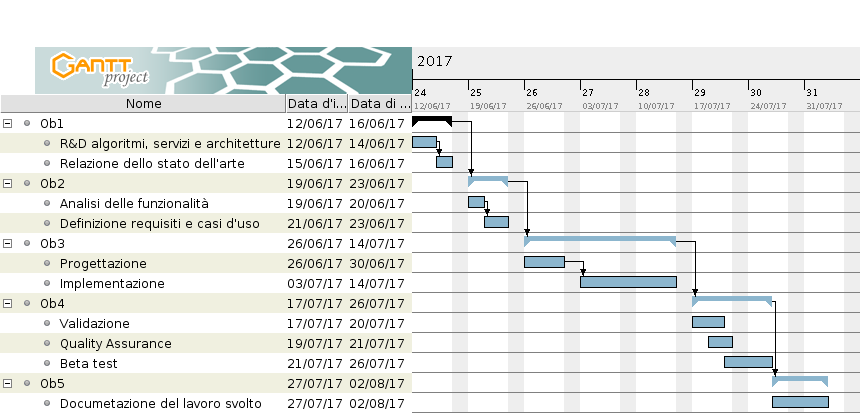
\includegraphics[height=8cm,width=15cm,keepaspectratio]{immagini/pianificazione-gantt}
      \caption{Diagramma di Gantt della pianificazione}
   \end{center}
\end{figure}

   \subsection{Strumenti utilizzati}
   Per ottenere buoni risultati durante la pianificazione \nomeAzienda{} utilizza GanttProject\footnote{Sito web del progetto GanttProject: \href{http://www.ganttproject.biz/}{www.ganttproject.biz}}, un software open-source per la realizzazione di diagrammi di \gls{Gantt} e \gls{PERT}. Il programma permette di costruire diagrammi con estrema facilità, gestendo scadenze, risorse, personale e dipendenze; inoltre permette di esportare il risultato in HTML o in formato PNG.\